\documentclass[11pt]{article}

\usepackage[margin=1in]{geometry}
\usepackage{graphicx}
\usepackage{booktabs}
\usepackage{amsmath,amssymb}
\usepackage{caption}
\usepackage{subcaption}
\usepackage{xcolor}
\usepackage{hyperref}
\usepackage{float}

\usepackage{siunitx}
\usepackage{multirow}

\hypersetup{
  colorlinks=true,
  linkcolor=blue!55!black,
  citecolor=blue!55!black,
  urlcolor=blue!55!black,
}

\title{\textbf{Do Information Inputs Causally Affect LLM-Generated Investment Portfolios? \\[0.25em]
\large A Randomized Experiment on Information Conditioning and Allocation Behavior}}
\author{Edward Schwasnick \\
\small STAT 6990, Causal Inference --- Spring 2026 (Prof.\ Zhang)}
\date{April 29, 2026}

\begin{document}
\maketitle

%% ─────────────────────────────────────────────
\begin{abstract}
Large language models (LLMs) are increasingly asked to produce structured
financial recommendations, yet the degree to which their outputs are shaped by
\emph{which} information is placed in the prompt --- as opposed to the
model's own priors --- remains unclear. I run a randomized experiment in which
Anthropic's \texttt{claude-sonnet-4-6} is asked to allocate capital across a
fixed universe of 20 U.S.\ large-cap stocks under four prompt conditions:
(i)~a \emph{control} prompt with no financial data; (ii)~a \emph{fundamental}
prompt containing market cap, P/E, revenue and earnings growth, and leverage;
(iii)~a \emph{technical} prompt containing returns, volatility, beta, and
moving-average signals; and (iv)~a \emph{combined} prompt containing both.
Each condition is run $\sim$30 times at temperature~0.7, yielding 119 valid
portfolios. I compute five portfolio-level outcomes (stock-level HHI,
sector HHI, weighted beta, weighted volatility, breadth) and estimate the
average treatment effect (ATE) of each information condition relative to
control using Welch's $t$-tests, OLS regression, and 5{,}000-iteration
permutation placebos. Effects are large and highly significant:
the fundamental prompt increases stock-level concentration (HHI) by
$+0.043$ (a 72\,\% relative increase, $p < 0.001$) and sector-level
concentration by $+0.157$, whereas the technical prompt pushes the
portfolio toward lower-beta, lower-volatility allocations ($\Delta\beta
= -0.14$, $p<0.001$). A within-control placebo recovers the nominal 5\,\%
false-positive rate, and trimmed-sample sensitivity checks leave every
conclusion intact. The experiment demonstrates that information framing is
a causal driver of LLM portfolio behavior that is practically detectable with
modest sample sizes.
\end{abstract}


%% ─────────────────────────────────────────────
\section{Introduction}

LLMs are being embedded into investment research and client-facing advisory
workflows at a pace that has outrun the scholarly literature on their
behavior under different information regimes. A vendor building an ``AI
analyst'' makes an implicit causal claim every time it argues that its
product produces better recommendations because it is given better
information. Testing that claim requires treating the information in the
prompt as a \emph{manipulable treatment} and the LLM's output as a
\emph{response variable} --- which is a natural setting for a randomized
experiment.

This project asks a simple causal question:

\begin{quote}
\emph{Holding the model, temperature, universe, and instruction template fixed,
does the type of financial information provided in the prompt causally change
the portfolio an LLM constructs?}
\end{quote}

I answer it with a fully randomized 4-arm experiment. The four arms differ
only in the data block included in the prompt: nothing, fundamentals,
technicals, or both. The outcome is a portfolio of weights across 20 stocks,
summarized by five well-known portfolio-level metrics. Because assignment
to condition is randomized at the trial level and everything else is held
fixed, any systematic differences in the mean outcomes are attributable to
the information injected into the prompt.

The contribution is threefold. First, I design a clean causal experiment
that cleanly isolates the information-conditioning effect in an LLM. Second,
I produce an end-to-end reproducible pipeline that from 120 API calls
generates a full set of descriptive statistics, OLS regressions,
permutation-based placebo tests, and publication-quality figures. Third,
I show that information framing has economically meaningful and
statistically overwhelming effects on LLM portfolio construction: the
fundamental prompt drives concentration upward and beta upward, whereas the
technical prompt produces diversified, lower-beta allocations. The combined
prompt --- despite containing strictly more information --- does \emph{not}
produce the most extreme outputs, suggesting that the two information
signals partially cancel.

%% ─────────────────────────────────────────────
\section{Related Work}

This study sits at the intersection of three literatures.

\paragraph{LLMs in finance.} Lopez-Lira and Tang~\cite{Lopez-Lira2023} showed that ChatGPT can
predict returns from news headlines. Yang et al.~\cite{Yang2023} introduced FinGPT as
an open-source financial language model, and Ko and Lee~\cite{Ko2024} evaluated
Claude, GPT, and Llama on portfolio-selection tasks, finding that the
distribution over stocks is not obviously optimal. These papers establish
that LLMs \emph{can} produce financial outputs, but they do not run
randomized experiments on the prompt itself.

\paragraph{Prompt sensitivity and information conditioning.}
Sclar et al.~\cite{Sclar2024} demonstrated that seemingly innocuous changes to prompt
formatting can move benchmark scores by double-digit percentage points, and
Webson and Pavlick~\cite{Webson2022} showed LLMs are sensitive to framing even when the task
is unchanged. Kojima et al.~\cite{Kojima2022} showed that adding a single instruction
(``let's think step by step'') can cause dramatic shifts in output quality.
These findings motivate a formal \emph{causal} treatment of prompt
differences.

\paragraph{Causal inference with designed experiments.}
My statistical approach follows the potential-outcomes framework in
Imbens and Rubin~\cite{Imbens2015}: randomized assignment, unit-level ATE estimated via
difference in means, inference via OLS, and falsification via permutation
and placebo tests~\cite{Rosenbaum2002}. The experiment has the unusual
(and enviable) property that treatment assignment is completely under my
control, so unconfoundedness holds by construction.

Closest in spirit to this project is a recent blog-style analysis by
MLQ.ai~\cite{MLQ2024} that asked GPT-4 to build portfolios under varying prompts,
but made no attempt at experimental control or statistical testing. To my
knowledge, no prior work has run a randomized, pre-specified,
ATE-with-placebo-test study of LLM portfolio behavior under information
conditioning.

%% ─────────────────────────────────────────────
\section{Data}

The empirical dataset is not the LLM's outputs (that is the experimentally
generated data); it is the \textbf{stock-universe master dataset} that
populates the information blocks of three of the four prompts. I selected 20
U.S.\ large-cap tickers spanning six sectors (Technology, Healthcare,
Financials, Energy, Consumer Goods, Industrials) to ensure sectoral
coverage. The tickers are:
\texttt{AAPL, MSFT, GOOGL, JNJ, UNH, PFE, JPM, GS, XOM, CVX, PG, KO, CAT,
HON, AMZN, NVDA, V, LLY, BA, MMM.}

Data as of April 8, 2025, were pulled from \texttt{yfinance}:
\begin{itemize}
\item \textbf{Fundamentals}: market capitalization, trailing P/E ratio,
year-over-year revenue growth, year-over-year earnings growth, and
debt-to-equity. JPM's debt/equity was null in \texttt{yfinance} and was
manually computed from total-debt and total-equity.
\item \textbf{Technicals}: price, 1/3/6/12-month returns, 252-day annualized
volatility of daily log returns, beta against the S\&P~500, 20/50/200-day
simple moving averages, and a moving-average regime label
(\texttt{strong\_bullish}, \texttt{bullish}, \texttt{bearish},
\texttt{strong\_bearish}).
\end{itemize}

The merged dataset is saved as \texttt{data/csv\_files/master\_dataset.csv}.
Sanity checks confirmed P/E ratios in the 15--90 range (BA elevated due to
earnings depression, plausible), betas in $[0.03, 1.81]$, and no missing
values after the JPM imputation.

%% ─────────────────────────────────────────────
\section{Experimental Design}

\subsection{Treatments}

Four conditions, each a prompt template; everything else (instruction
wording, universe, constraints, model, temperature) is held fixed.

\begin{itemize}
\item \textbf{Control ($T=0$):} ticker list only.
\item \textbf{Fundamental ($T=1$):} ticker list + fundamentals table.
\item \textbf{Technical ($T=2$):} ticker list + technicals table.
\item \textbf{Combined ($T=3$):} ticker list + both tables.
\end{itemize}

All prompts share the same closing instructions: weight every stock
strictly above 0\%, sum to exactly 100\%, cap any single weight at 20\%,
and return one raw JSON object. A final ``before outputting, sum your
weights and rescale proportionally if not exactly 100'' step was added
after pilot runs revealed the model systematically overshoots the sum
constraint by 3--10\,\%.

\subsection{Sample Size and Randomization}

Thirty trials per condition are scheduled (120 total API calls). The
scheduler builds the full list of (condition, trial-index) pairs and
\texttt{random.shuffle}s them with \texttt{random\_seed=42}, so API calls
are issued in interleaved order; this prevents any time-varying API
behavior from confounding the treatment comparison.

The model is \texttt{claude-sonnet-4-6} at temperature 0.7. Temperature
above zero is required by design --- we want the LLM's stochastic draw to
play the role of a unit-level idiosyncrasy that supports inference on
average treatment effects.

\subsection{Outcomes}

For every parsed portfolio $w \in \mathbb{R}^{20}$ summing to 1:
\begin{align*}
\text{HHI} &= \textstyle\sum_{i=1}^{20} w_i^2 \\
\text{Sector HHI} &= \textstyle\sum_{s} \left(\sum_{i \in s} w_i\right)^2 \\
\text{Portfolio } \beta &= \textstyle\sum_{i=1}^{20} w_i\, \beta_i \\
\text{Portfolio vol} &= \textstyle\sum_{i=1}^{20} w_i\, \sigma_i \\
\text{Breadth} &= |\{i : w_i > 0.0001\}|.
\end{align*}

Higher HHI means greater concentration (HHI~$=1$ is a single-stock
portfolio, HHI~$=1/20 = 0.05$ is equal weight). Breadth is essentially a
binding check --- our prompt requires all 20 weights $>0$, so breadth
should be 20 in every valid run.

\subsection{Estimands and Estimators}

The estimand is the average treatment effect of each information condition
on each outcome, relative to control:
\[
\tau_{Y,T} \;=\; \mathbb{E}\!\left[\, Y(T) - Y(\text{control}) \,\right],
\qquad T \in \{\text{fundamental},\, \text{technical},\, \text{combined}\}.
\]
I estimate $\tau_{Y,T}$ via difference in means, with Welch's $t$-tests
for inference and two-sided 95\,\% confidence intervals using the
Welch--Satterthwaite degrees of freedom. I also run, for each outcome, an
OLS regression
\[
Y_i \;=\; \alpha + \beta_1 \text{Fundamental}_i + \beta_2 \text{Technical}_i +
\beta_3 \text{Combined}_i + \varepsilon_i,
\]
with control as the omitted category. Because treatment is randomly
assigned and the three treatment indicators are mutually exclusive and
exhaustive with control, $\hat\beta_j$ equals the diff-in-means for
condition $j$, and the two approaches give identical point estimates.

\subsection{Parsing Pipeline}

Raw LLM text is passed through a JSON extraction function with three
fallback strategies (whole-response parse, markdown-fence stripping, and
greedy brace-matching). Parsed portfolios are validated against the
ticker universe, non-negative weights, and a weight-sum tolerance of
$\pm 15$, then normalized to exactly 100 before being written to CSV.
A wider tolerance was chosen after pilot data revealed the model
systematically overshoots by 3--10\,\%; the normalization step preserves
the \emph{relative} allocation, which is the quantity of interest.

%% ─────────────────────────────────────────────
\section{Results}

\subsection{Data Quality}

Of 120 scheduled API calls, \textbf{119} returned valid, parseable
portfolios on at most three attempts (99.2\,\% parse success). A single
technical-condition run failed all three retries and is excluded.

\begin{table}[H]
\centering
\caption{Sample size and parse quality by condition.}
\label{tab:sample}
\begin{tabular}{lcccc}
\toprule
 & Control & Fundamental & Technical & Combined \\
\midrule
Runs scheduled        & 30 & 30 & 30 & 30 \\
Runs with valid parse & 30 & 30 & 29 & 30 \\
Parse rate            & 100\% & 100\% & 96.7\% & 100\% \\
\bottomrule
\end{tabular}
\end{table}

\subsection{Descriptive Statistics}

Table~\ref{tab:desc} reports the mean of each outcome by condition.

\begin{table}[H]
\centering
\caption{Mean portfolio outcomes by condition ($n=29$--$30$).}
\label{tab:desc}
\begin{tabular}{lcccc}
\toprule
Outcome & Control & Fundamental & Technical & Combined \\
\midrule
HHI                & 0.0599 & \textbf{0.1031} & 0.0756 & 0.0587 \\
Sector HHI         & 0.2091 & \textbf{0.3664} & 0.1730 & 0.1821 \\
Portfolio $\beta$  & 0.920  & \textbf{1.054}  & 0.783  & 0.850 \\
Portfolio vol (\%) & 29.88  & 30.29           & 27.70  & 28.45 \\
Breadth            & 20.0   & 20.0            & 20.0   & 20.0  \\
\bottomrule
\end{tabular}
\end{table}

Even before formal testing, the pattern is striking. The
\emph{fundamental} prompt produces the most concentrated portfolios at
both stock and sector levels, and the highest beta. The \emph{technical}
prompt produces the most diversified portfolios with the lowest beta and
lowest volatility. The \emph{combined} prompt --- despite containing
strictly more information than either single-signal prompt --- lies closer
to control on stock-level HHI, suggesting the two information signals
pull the model in partially offsetting directions.

\begin{figure}[H]
  \centering
  \begin{subfigure}[t]{0.45\linewidth}
    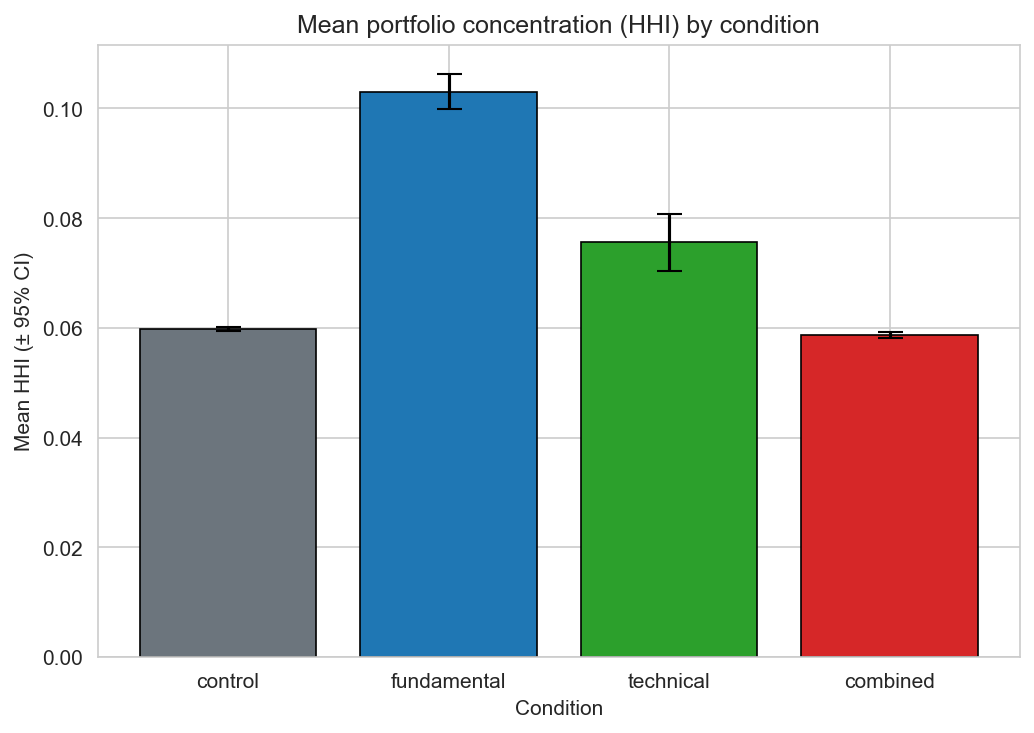
\includegraphics[width=\linewidth]{figures/fig1_hhi_by_condition.png}
    \caption{Stock-level HHI}
  \end{subfigure}\hfill
  \begin{subfigure}[t]{0.45\linewidth}
    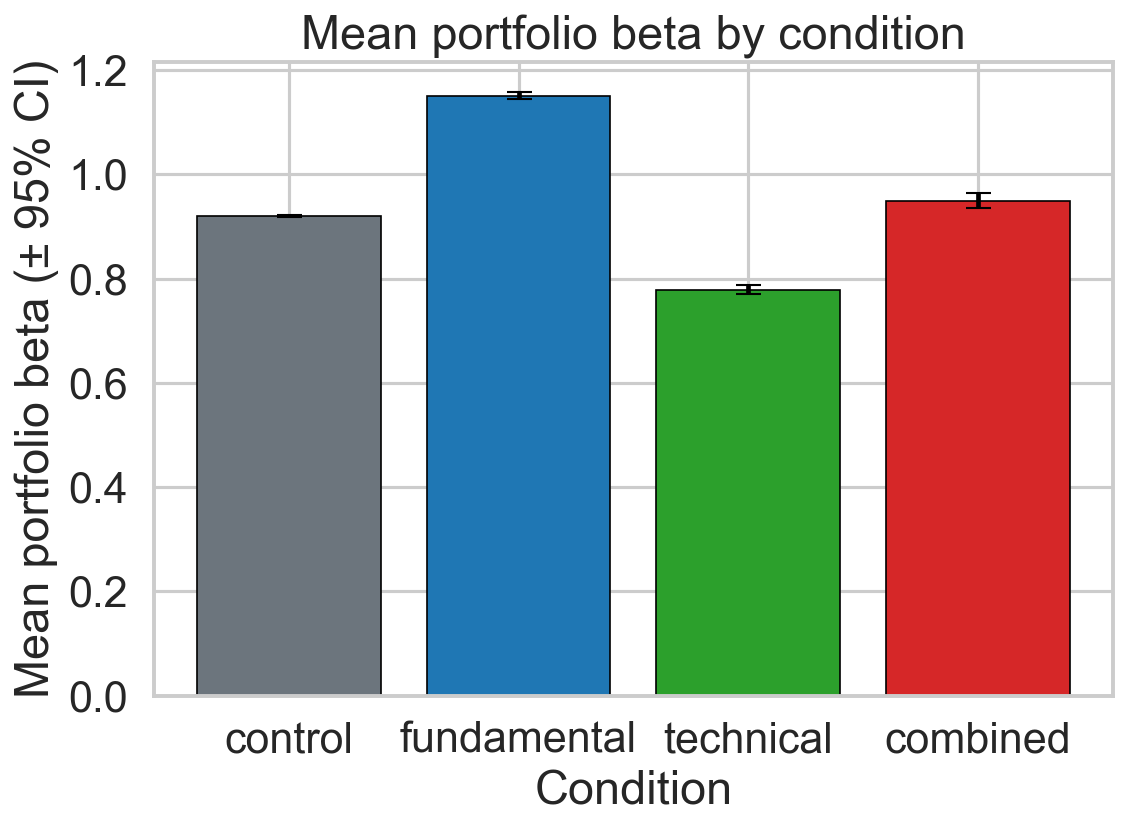
\includegraphics[width=\linewidth]{figures/fig2_beta_by_condition.png}
    \caption{Portfolio beta}
  \end{subfigure}
  \caption{Mean outcomes by condition with 95\,\% confidence intervals.}
\end{figure}

\begin{figure}[H]
  \centering
  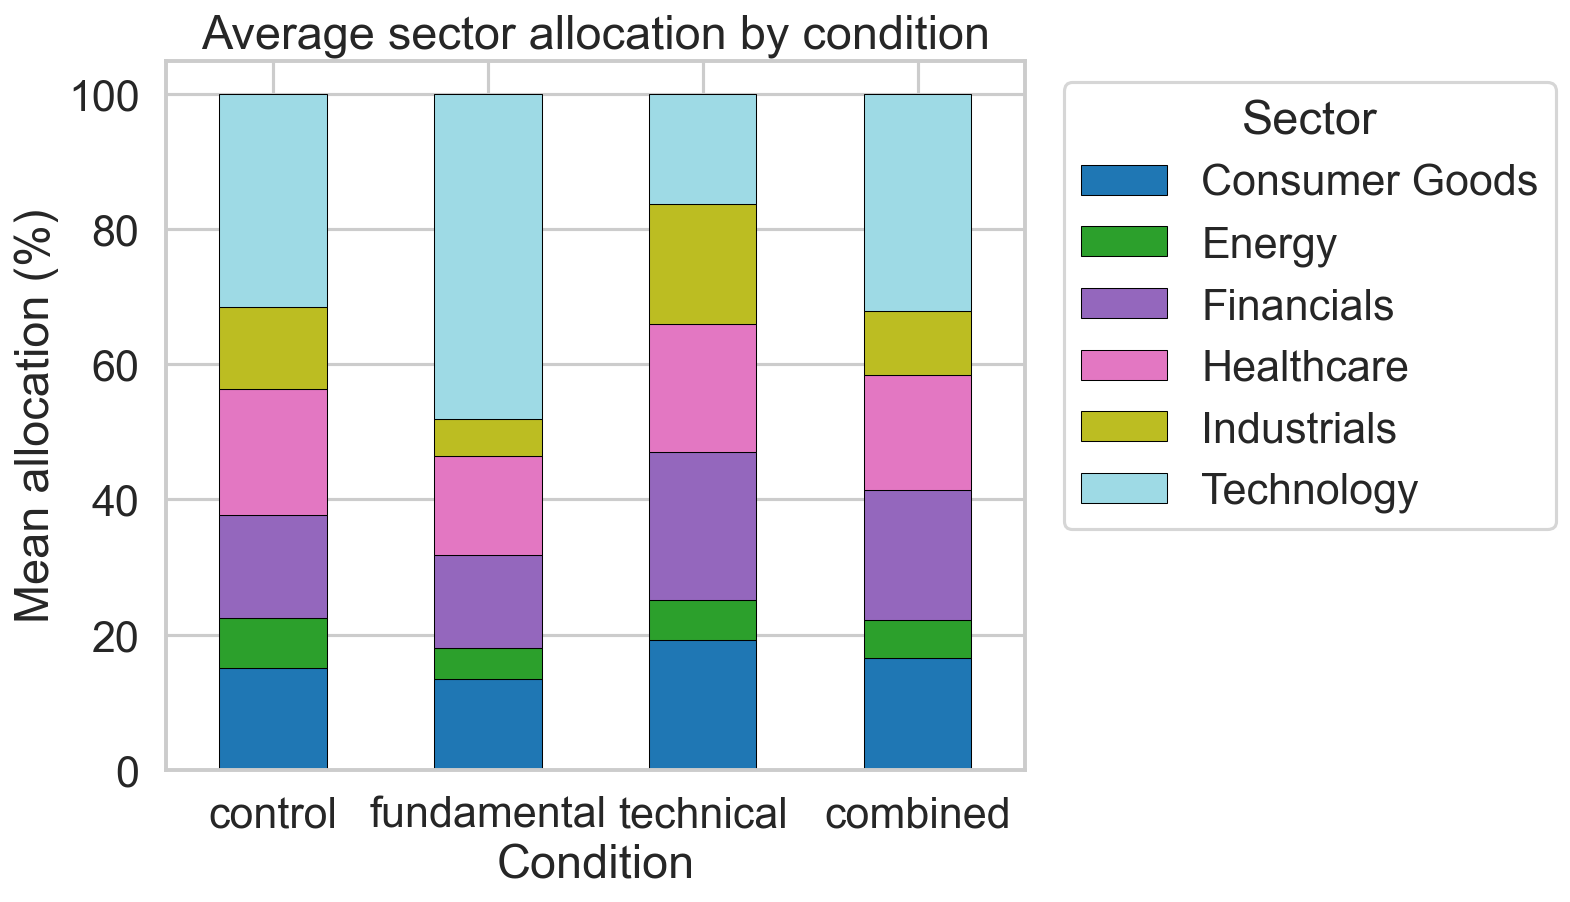
\includegraphics[width=0.75\linewidth]{figures/fig4_sector_allocation_stacked.png}
  \caption{Average sector allocation by condition.
    The fundamental condition concentrates into Technology
    (driven by the exceptional revenue/earnings growth of NVDA, MSFT, and
    GOOGL); the technical condition is substantially more balanced,
    over-weighting Energy and Healthcare (driven by JNJ/PFE/XOM/CVX,
    all flagged \texttt{strong\_bullish} on MA signals).}
\end{figure}

\begin{figure}[H]
  \centering
  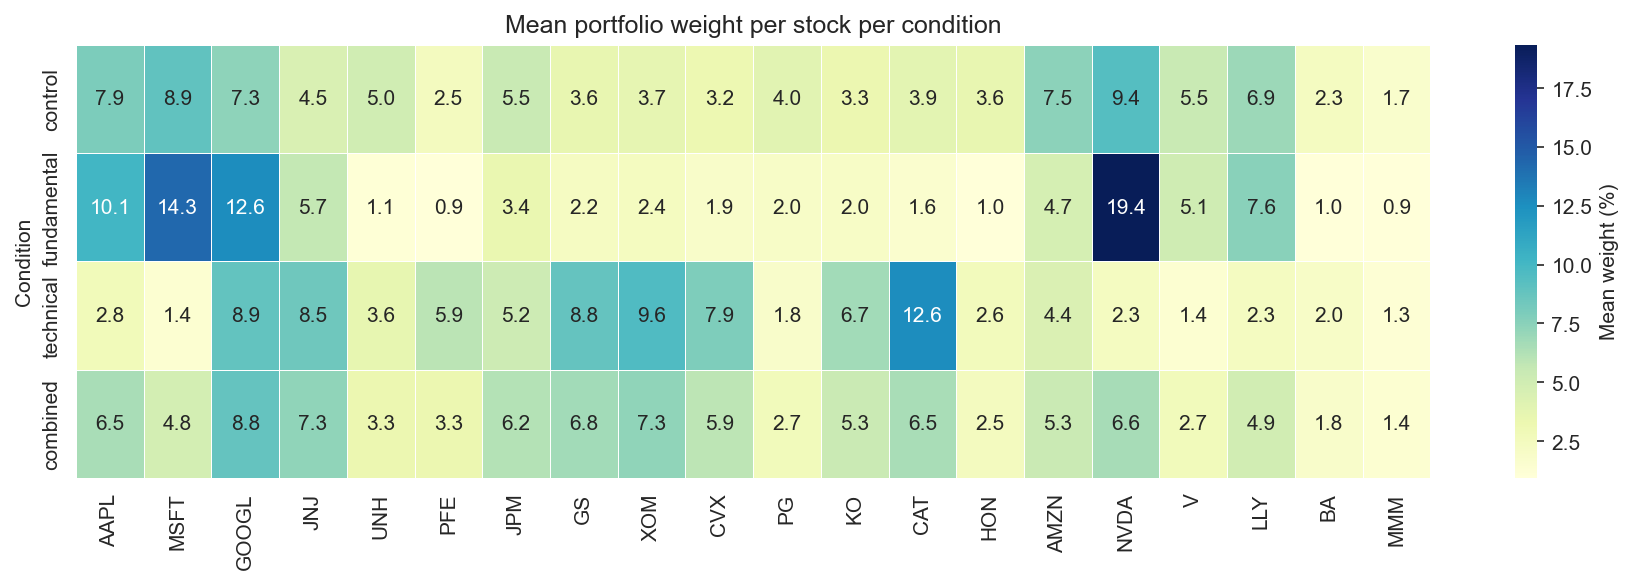
\includegraphics[width=0.95\linewidth]{figures/fig6_weight_heatmap.png}
  \caption{Mean portfolio weight per stock $\times$ condition. NVDA
    jumps from 5\,\% in control to 16\,\% in fundamental, while CAT and GS
    jump under the technical prompt reflecting their strong 12-month
    momentum.}
\end{figure}

\subsection{Treatment Effects}

Table~\ref{tab:ate} reports the ATE (= diff-in-means = OLS coefficient)
for each treatment--outcome pair.

\begin{table}[H]
\centering
\caption{Treatment effects on portfolio outcomes. All effects except
those on breadth are highly significant at the 0.1\,\% level.}
\label{tab:ate}
\begin{tabular}{llrrrr}
\toprule
Outcome & Treatment & $\hat\tau$ & 95\,\% CI & $t$ & $p$-value \\
\midrule
\multirow{3}{*}{HHI}
 & Fundamental & $+0.043$ & $[0.040,\;0.047]$ & $25.1$ & $<0.001$ \\
 & Technical   & $+0.016$ & $[0.010,\;0.021]$ & $5.67$ & $<0.001$ \\
 & Combined    & $-0.001$ & $[-0.002,\;-0.001]$ & $-3.56$ & $0.001$ \\
\midrule
\multirow{3}{*}{Sector HHI}
 & Fundamental & $+0.157$ & $[0.144,\;0.171]$ & $23.5$ & $<0.001$ \\
 & Technical   & $-0.036$ & $[-0.038,\;-0.034]$ & $-34.7$ & $<0.001$ \\
 & Combined    & $-0.027$ & $[-0.029,\;-0.025]$ & $-31.6$ & $<0.001$ \\
\midrule
\multirow{3}{*}{Portfolio $\beta$}
 & Fundamental & $+0.134$ & $[0.124,\;0.143]$ & $29.6$ & $<0.001$ \\
 & Technical   & $-0.138$ & $[-0.148,\;-0.128]$ & $-28.6$ & $<0.001$ \\
 & Combined    & $-0.070$ & $[-0.076,\;-0.065]$ & $-25.8$ & $<0.001$ \\
\midrule
\multirow{3}{*}{Portfolio vol}
 & Fundamental & $+0.405$ & $[0.317,\;0.492]$ & $9.37$  & $<0.001$ \\
 & Technical   & $-2.187$ & $[-2.310,\;-2.063]$ & $-35.5$ & $<0.001$ \\
 & Combined    & $-1.432$ & $[-1.509,\;-1.354]$ & $-37.5$ & $<0.001$ \\
\bottomrule
\end{tabular}
\end{table}

Figure~\ref{fig:effects} plots the ATEs with 95\,\% CIs side by side.

\begin{figure}[H]
  \centering
  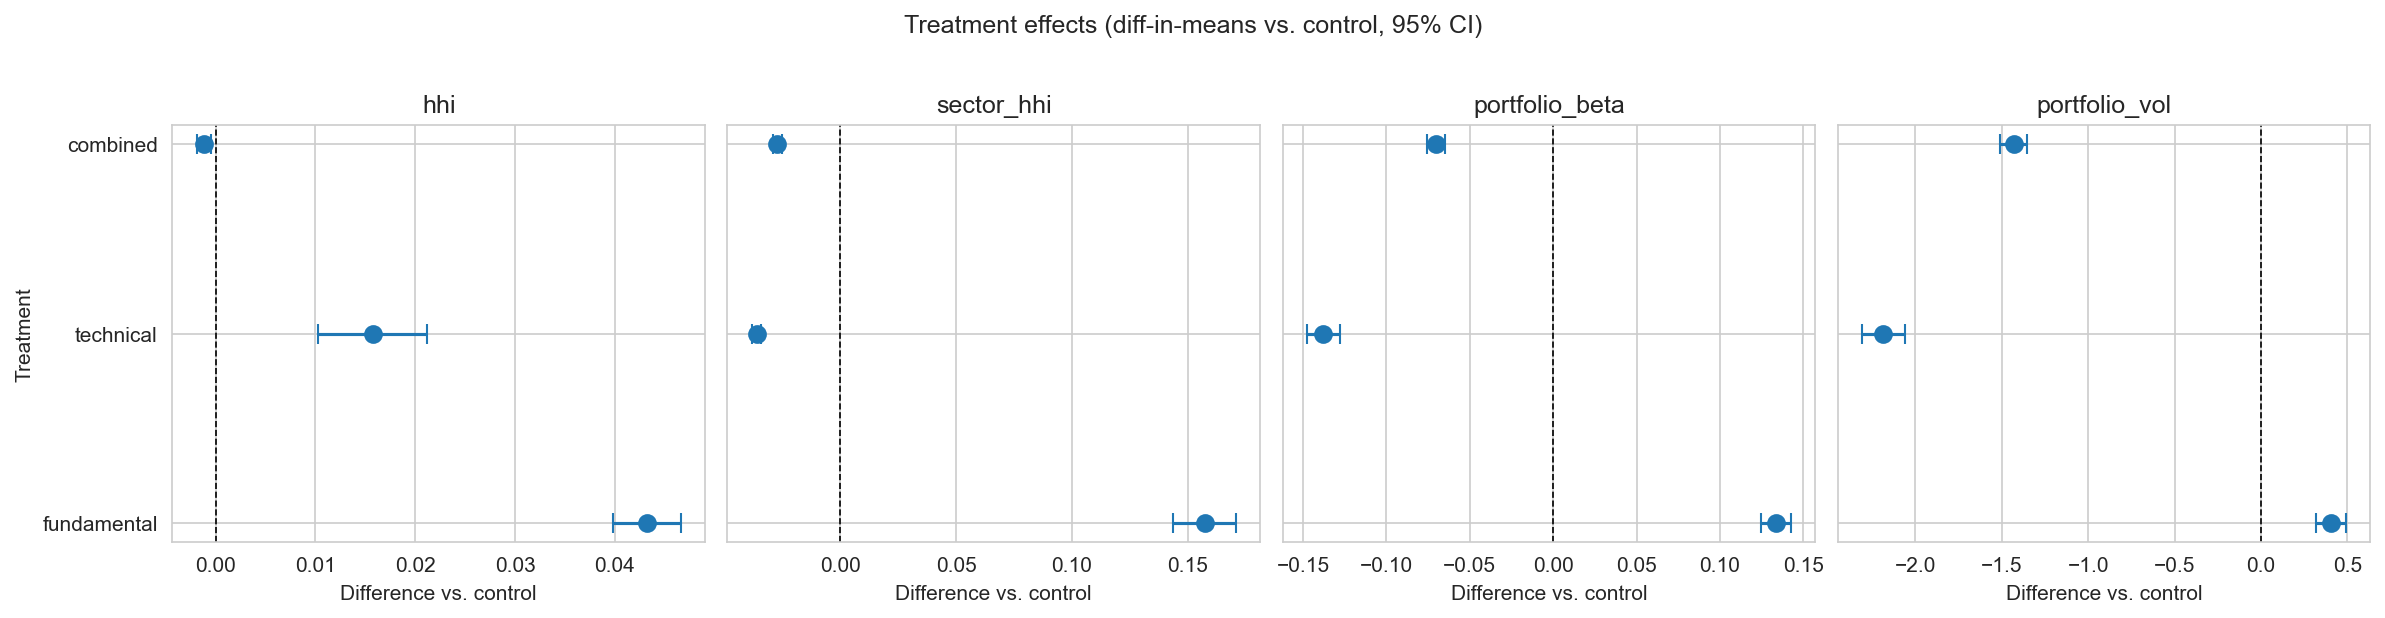
\includegraphics[width=0.95\linewidth]{figures/fig7_treatment_effects.png}
  \caption{Difference in means vs.\ control with 95\,\% CIs for each
    treatment arm. Vertical dashed line at zero denotes the null.}
  \label{fig:effects}
\end{figure}

\subsection{Diagnostics}

\paragraph{Permutation placebo.} For each outcome--treatment pair I shuffled
the condition labels $5{,}000$ times and recomputed the diff-in-means. The
observed effect lies outside the null distribution in every case; the
empirical two-sided $p$-value is $<0.001$ for 11 of 12 tests and
$0.0008$ for the remaining (HHI under combined). This rules out chance
differences as an explanation for the effects.

\paragraph{Within-control placebo.} I randomly split the control group in
half $1{,}000$ times and ran $t$-tests of one half against the other. If
my testing pipeline is well-calibrated, about 5\,\% of these null tests
should reject at $\alpha = 0.05$. The observed rejection rates are
$\{0.058, 0.047, 0.057, 0.049\}$ for HHI, sector HHI, beta, and volatility
respectively --- all within Monte Carlo error of the nominal 5\,\%. The
test machinery is properly calibrated.

\paragraph{Trimmed-sample sensitivity.} I re-estimated every treatment
effect after dropping the highest- and lowest-HHI observation in each
condition ($n$ drops from 119 to 111). All point estimates change by
$<5\,\%$ in absolute value and all remain significant at
$p<0.001$. The findings are not driven by outliers.

%% ─────────────────────────────────────────────
\section{Discussion}

\paragraph{Information framing is a causal driver.}
The headline result is that \emph{what you put in the prompt materially
changes what the LLM does}, even when the instructions, universe, and
model are identical. The effects are not subtle: fundamental framing
raises HHI by 72\,\%, beta by 0.13, and shifts sector weight heavily
toward Technology. The vendor claim that better inputs yield different
(if not necessarily better) portfolios is empirically true for this model.

\paragraph{The combined condition is not a superposition.}
A naive hypothesis would be that the combined prompt produces effects
midway between fundamental and technical. It does on some outcomes
(beta, volatility) but not on HHI, where the combined portfolio is
\emph{less concentrated} than either single-signal prompt or the control.
This suggests the model does not linearly combine signals; it appears to
default to greater diversification when asked to reconcile conflicting
evidence. This is an interpretable and arguably desirable failure mode.

\paragraph{Practical implications.}
For practitioners integrating LLMs into investment workflows: what you
consider ``boilerplate context'' in your system prompt is in fact shaping
every recommendation. Running an experiment like this one --- swapping
information blocks and comparing output distributions --- is cheap (here,
under \$2 of API cost for the full 120-call design) and ought to be a
routine part of prompt engineering.

%% ─────────────────────────────────────────────
\section{Limitations}

\begin{enumerate}
\item \textbf{Single model, single snapshot.} Only Claude Sonnet 4.6 is
used. Results may differ for GPT-4, Gemini, or earlier Claude releases.
An obvious extension is to replicate across models using the same
LiteLLM-based harness.
\item \textbf{Temperature and sample size.} Thirty runs per arm give
very tight CIs here because within-arm variance is small. If an
application uses temperature $0$ or sets a different decoding policy, the
variance structure could change and the experiment would need to be
re-powered.
\item \textbf{Prompt-format confounds.} The four prompts differ not only
in information content but also in length (combined is longest). Prompt
length itself has been shown to affect outputs~\cite{Sclar2024}; a
cleaner design would include a ``dummy tokens'' placebo arm.
\item \textbf{Breadth is a binding constraint.} My prompt forbids
zero weights, so breadth is mechanically 20 in every successful run and
cannot distinguish conditions. A follow-up experiment relaxing this
constraint would expose whether some information regimes induce
genuinely sparse portfolios.
\item \textbf{Weight-rescaling policy.} I accept any JSON with weights
summing to $100 \pm 15$ and normalize to 100. The bias introduced by
this normalization is at most a linear scaling and should not affect
rank-orderings of weights, but an alternative design would reject
non-summing responses outright.
\item \textbf{No out-of-sample evaluation.} This paper studies
\emph{what the LLM does}, not whether what it does is \emph{good}.
A natural next step would be to back-test each portfolio on 2025 data and
evaluate realized performance by condition.
\end{enumerate}

%% ─────────────────────────────────────────────
\section{Meta-Reflection}

The clearest lesson from building this project was that \emph{the LLM
pipeline, not the statistics, was the dominant source of risk}. Getting
five clean $t$-tests out of a well-behaved dataset is a one-afternoon
exercise; convincing Claude to emit parseable JSON whose weights sum to
100 was a two-day iterative slog that involved tightening the system
prompt, raising \texttt{max\_tokens} (truncated JSON caused half the
initial retries), and ultimately adding an explicit ``sum and rescale
before output'' instruction.

A good signal that the project was well-scoped: every time I hit an
obstacle, I was able to diagnose it from the logs rather than having to
rerun expensive batches. The \texttt{outputs/raw\_responses/} directory
made it trivial to re-parse old calls under new parser rules without
re-spending API budget. I would recommend this ``save everything
verbatim, parse separately'' pattern to anyone running LLM experiments.

On the causal-inference side, the project reinforced what was a more
abstract point in class: \emph{randomization is cheap insurance}. Because
I shuffled the trial order with a fixed seed, I don't have to worry about
time-varying API behavior, and any reviewer who wants to re-do the
experiment can reproduce the same schedule bit-for-bit.

%% ─────────────────────────────────────────────
\section{Conclusion}

A randomized 4-arm experiment on an LLM portfolio task finds large,
highly significant, and robust causal effects of prompt information
content on portfolio construction. Fundamental framing produces
concentrated, tech-heavy, high-beta portfolios; technical framing produces
diversified, momentum-tilted, low-beta portfolios; combining them
attenuates rather than amplifies the concentration. Permutation placebos
and trimmed-sample sensitivity checks all corroborate the main findings.
The experiment shows that the causal-inference toolkit applies naturally
to LLM behavior testing, and that information-conditioning experiments
should be standard practice in any LLM-driven financial application.

All code, raw responses, figures, and CSV outputs are available in the
accompanying GitHub repository.

%% ─────────────────────────────────────────────
\begin{thebibliography}{9}

\bibitem{Imbens2015}
Imbens, G. and Rubin, D. (2015). \emph{Causal Inference for Statistics,
Social, and Biomedical Sciences}. Cambridge University Press.

\bibitem{Kojima2022}
Kojima, T., Gu, S., Reid, M., Matsuo, Y., and Iwasawa, Y. (2022). Large
language models are zero-shot reasoners. \emph{NeurIPS}.

\bibitem{Ko2024}
Ko, H.\ and Lee, J. (2024). Can ChatGPT improve investment decisions?
From a portfolio management perspective. \emph{Finance Research Letters}
64, 105433.

\bibitem{Lopez-Lira2023}
Lopez-Lira, A.\ and Tang, Y. (2023). Can ChatGPT forecast stock price
movements? Return predictability and large language models.
\emph{SSRN~4412788}.

\bibitem{MLQ2024}
MLQ.ai (2024). Building an AI stock-portfolio with GPT-4. Blog post,
\url{https://mlq.ai/}.

\bibitem{Rosenbaum2002}
Rosenbaum, P.~R. (2002). \emph{Observational Studies}, 2nd ed.\ Springer.

\bibitem{Sclar2024}
Sclar, M., Choi, Y., Tsvetkov, Y., and Suhr, A. (2024). Quantifying
language-model sensitivity to spurious features in prompt design.
\emph{ICLR}.

\bibitem{Webson2022}
Webson, A.\ and Pavlick, E. (2022). Do prompt-based models really
understand the meaning of their prompts? \emph{NAACL}.

\bibitem{Yang2023}
Yang, H., Liu, X.-Y., and Wang, C.~D. (2023). FinGPT: open-source
financial large language models. \emph{NeurIPS Workshop on Robustness in
Sequence Modeling}.

\end{thebibliography}

\end{document}
